% Number 280
% CVPMA Algebra Units
% Dune buggy overtaking, find distance
% JG

% Watermark
\AddToShipoutPicture*{\BackgroundPic}

\addtocounter {ProbNum} {1}

%\begin{floatingfigure}[r]{.3\textwidth}
%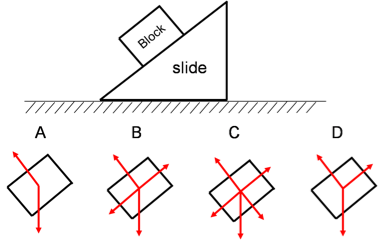
\includegraphics[scale=.4]{/Users/jgates/desktop/latex/pics/incline3.png}
%\end{floatingfigure}
 
{\bf \Large{\arabic{ProbNum}}}A dune buggy takes off down the beach, driving ${8.9~\tfrac{m}{s}}$.  It then passes a second dune buggy, which sets off after it at a speed of ${12.1~\tfrac{m}{s}}$, after waiting four seconds to start.

\bigskip
Describe some ways in which a CVPM model of this situation would not match reality.

\vspace{30 mm}
How far has the first dune buggy traveled when it is caught by the second dune buggy?

%\begin{center}
%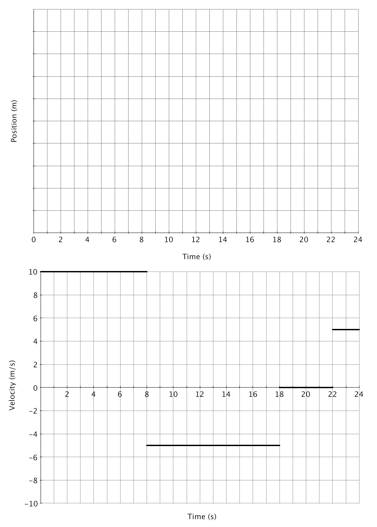
\includegraphics[scale=.77]{/Users/jgates/desktop/latex/pics/vtoxgraph1.png}
%\end{center}
 
\vfill

\newpage